\documentclass[10pt,twocolumn]{article}
\usepackage[margin=0.72in]{geometry}
\usepackage{times}
\usepackage{microtype}
\usepackage{graphicx}
\usepackage{booktabs}
\usepackage{amsmath,amssymb}
\usepackage{xcolor}
\usepackage{hyperref}
\usepackage{algorithm}
\usepackage{algpseudocode}
\usepackage{caption}
\usepackage{subcaption}
\usepackage{enumitem}
\hypersetup{colorlinks=true,linkcolor=black,citecolor=teal,urlcolor=blue}
\captionsetup{font=small,labelfont=bf}
\setlist[itemize]{leftmargin=*,nosep}
\newcommand{\method}{Density-Aware Adaptive SoM}
\newcommand{\best}[1]{\textbf{#1}}

\title{\vspace{-0.35in}\textbf{When Does Visual Prompting Help or Hurt Edge MLLMs? Occlusion Trade-offs and Density-Aware Adaptation}}
\author{Lei Pan\\
School of Artificial Intelligence, Jilin University, Changchun, China\\
\texttt{panlei9925@mails.jlu.edu.cn}\thanks{Code: \url{https://github.com/LeiPan-JLU/adaptive-visual-prompting-mllm}; Project page: \url{https://leipan-jlu.github.io}}}
\date{November 2026}

\begin{document}
\maketitle

\begin{abstract}
Training-free visual prompting is attractive for edge multimodal large language models (MLLMs), yet the Set-of-Mark (SoM) recipe was designed for large proprietary models with dense annotation budgets. We report a controlled diagnostic study on Qwen2-VL-2B-Instruct with 400 CV-Bench 2D questions, rather than claiming a new state of the art. Two empirical findings emerge. First, \emph{task--prompt decoupling}: a simple $3\times3$ coordinate Grid improves 2D spatial relation accuracy to 66.5\% from 61.0\% for the raw image and reaches 63.2\% overall, without occluding the objects; in contrast, every detector-based SoM variant remains below the raw image on 2D counting (Raw 62.0\%; Adaptive 59.0\%; Naive 55.0\%). Second, an \emph{occlusion trade-off} coupled with \emph{class-agnostic detector distraction}: fixed thick boxes and opaque tags significantly hurt the 2B model (Naive 56.8\% vs.\ Raw 61.5\%, $p=0.0163$), especially at medium density (49.7\%). Density-aware rendering recovers most of this loss (62.0\% vs.\ 56.8\%, $p=0.0038$; medium 60.0\% vs.\ 49.7\%, $p=0.0015$), but it does not exceed the raw image ($p=0.8642$) because a category-agnostic detector can still place labels on irrelevant objects (e.g., bananas when the question asks about bowls). The study is training-free, adds no parameters, and runs in about 4.4\,GB on an 8\,GB laptop GPU.
\end{abstract}

\section{Introduction}
\label{sec:intro}
Multimodal large language models are increasingly deployed on consumer hardware, but small open models still struggle with fine-grained counting and spatial relations. Qwen2-VL-2B-Instruct is a representative edge model: it accepts arbitrary-resolution images and fits in an 8\,GB GPU when the visual token budget is capped, yet dense scenes remain difficult.

Set-of-Mark prompting improves visual grounding by drawing numbered marks on candidate regions. The original recipe assumes a strong segmentation proposal engine and a large model that can tolerate substantial overlay. On a 2B model, a thick box and a large opaque tag may hide the object boundary or the gap between two objects, which is exactly the evidence needed for counting and ``left of / above'' questions. This creates an \emph{occlusion trade-off}: annotations can help localization while simultaneously destroying the visual signal.

We therefore treat visual prompting as an empirical diagnosis problem. Our contributions are:
\begin{itemize}
\item A fixed, controlled 400-question CV-Bench 2D protocol (200 counting, 200 relation) that compares Raw, Grid, Naive SoM, and Adaptive SoM under identical questions and images on a 2B edge model.
\item Two findings with clear boundaries: (i) \emph{task--prompt decoupling}---Grid helps spatial relation, while no detector-based SoM beats Raw on counting; (ii) \emph{occlusion trade-off plus class-agnostic detector distraction}---fixed SoM hurts, density-aware rendering recovers, but neither fixes labels placed on irrelevant objects.
\item \method{}, a training-free renderer that uses object count $N$ and union box-area ratio $\rho$ to switch among three annotation regimes, with an open-source implementation and reproducible logs.
\end{itemize}

\begin{figure*}[t]
\centering
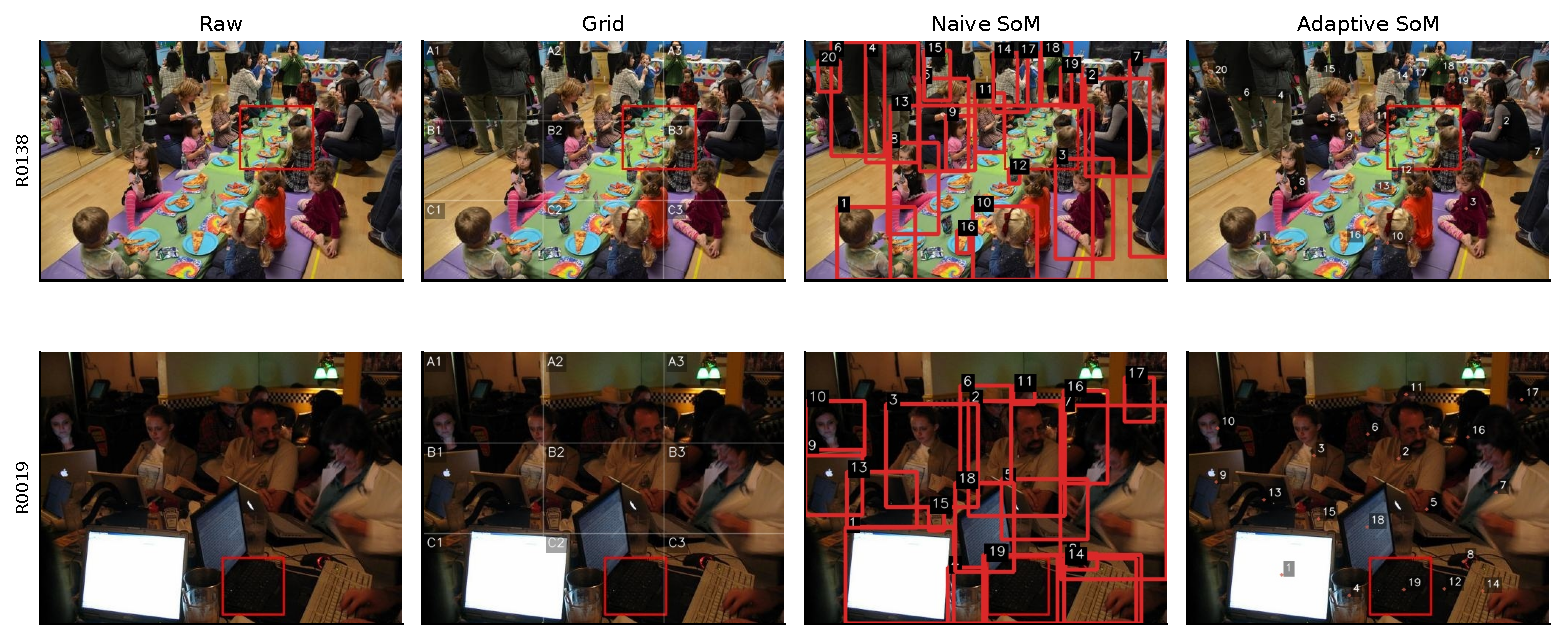
\includegraphics[width=0.98\textwidth]{figures/fig1_method_overview.pdf}
\caption{Four input conditions on two high-density CV-Bench examples. Naive SoM uses fixed thick boxes and opaque tags; Adaptive SoM reduces the annotation footprint as density grows. The model receives the same question in all conditions.}
\label{fig:overview}
\end{figure*}

\section{Related Work}
\label{sec:related}
\paragraph{Edge multimodal LLMs.}
LLaVA-1.5 established a strong open visual-instruction baseline \cite{liu2024llava15}, while Qwen2-VL adds dynamic-resolution vision encoding for images of arbitrary aspect ratio \cite{wang2024qwen2vl}. Cambrian-1 explores vision-centric MLLM design and introduces CV-Bench \cite{tong2024cambrian}; BLINK shows that many MLLMs can see but still fail at fine-grained perception \cite{fu2024blink}. These results motivate testing perception aids on a 2B model rather than assuming that a larger model's prompting recipe transfers.

\paragraph{Training-free visual prompting.}
Set-of-Mark overlays numbered masks or boxes and substantially improves grounding in GPT-4V \cite{yang2023setofmark}. Red-circle prompting studies visual prompt engineering for VLMs \cite{shtedritski2023redcircle}; Visual Sketchpad uses sketches as a visual chain of thought \cite{hu2024sketchpad}; See\&Trek studies training-free spatial prompting \cite{seetrek2025}; and recent work asks whether MLLMs know where to look for small details \cite{zhang2025mllmsknow}. Unlike this line of work, we quantify when marks help and when a detector's category-agnostic proposals become distractors on an edge model.

\paragraph{Inference-time hallucination and spatial reasoning.}
POPE evaluates object hallucination \cite{li2023pope}; VCD and OPERA mitigate hallucination through contrastive decoding and over-trust penalties \cite{leng2024vcd,huang2024opera}; test-time hallucination control remains an active direction \cite{tth2026}; and Visual-RFT explores reinforcement fine-tuning as an alternative to training-free prompting \cite{liu2025visualrft}. Our study is complementary: it holds the model fixed, uses no extra training, and diagnoses the interaction between annotation density and task type.

\section{Method}
\label{sec:method}
\paragraph{Proposals and density.}
For an image of size $W\times H$, YOLOv8n \cite{jocher2023yolov8} produces boxes $B=\{b_i\}_{i=1}^{N}$ at confidence 0.25 (class-agnostic, capped at 20). If no box is returned, a conservative Canny-contour fallback supplies proposals; this is needed for icon-like ADE20K images outside the COCO vocabulary. Let $M=\bigcup_i b_i$ be the union mask. We define
\begin{equation}
\rho = \frac{1}{WH}\sum_{x=1}^{W}\sum_{y=1}^{H}\mathbf{1}\left[(x,y)\in M\right].
\end{equation}
The density level is
\begin{equation}
\ell(N,\rho)=
\begin{cases}
\text{Low}, & N\le 3 \ \text{and}\ \rho<0.35,\\
\text{Medium}, & N\in[4,8]\ \text{or}\ 0.35\le\rho<0.60,\\
\text{High}, & N\ge 9\ \text{or}\ \rho\ge0.60.
\end{cases}
\end{equation}

\paragraph{Rendering.}
Low density uses a translucent coloured box (alpha 0.55) and a small corner tag. Medium density uses a one-pixel translucent outline (alpha 0.35) and a compact in-box tag. High density removes boxes and draws a translucent centre dot with a micro tag, minimizing occlusion. Naive SoM uses a 3\,px red box and an opaque black tag at every proposal; Grid overlays a 3$\times$3 coordinate grid with A1--C3 labels. All conditions are rendered at the original image resolution and saved as JPEG quality 95.

\begin{algorithm}[t]
\caption{Density-aware visual prompting}
\label{alg:avp}
\begin{algorithmic}[1]
\Require image $I$, detector $f$, thresholds in Eq.~2
\State $B \gets f(I)$ \Comment{YOLOv8n, conf 0.25, max 20}
\If{$B=\varnothing$}
    \State $B\gets$ contour proposals
\EndIf
\State $N\gets|B|$; compute union mask $M$ and $\rho$
\State $\ell\gets$ density level from Eq.~2
\If{$\ell=$ Low}
    \State draw translucent boxes and corner tags
\ElsIf{$\ell=$ Medium}
    \State draw 1\,px outlines and compact tags
\Else
    \State draw centre dots and micro tags
\EndIf
\State \Return rendered image
\end{algorithmic}
\end{algorithm}

\section{Experiments}
\label{sec:exp}
\paragraph{Setup.}
We use the 2D split of CV-Bench and sample 200 Count and 200 Relation questions with seed 42 (400 total). The model is Qwen2-VL-2B-Instruct in float16 on an NVIDIA RTX 5060 Laptop GPU (8\,GB). The processor uses min/max pixels $256\times28^2$ and $512\times28^2$; decoding is greedy with at most 32 new tokens. Each condition uses the same question and the same image content, differing only in the overlay. We report accuracy with 95\% Wilson intervals, mean latency, and exact McNemar tests on paired predictions.

\begin{table}[t]
\centering
\small
\setlength{\tabcolsep}{3.2pt}
\begin{tabular}{lcccc}
\toprule
Method & Overall & Count & Relation & Lat. (s) \\
\midrule
Raw & 61.5 & \best{62.0} & 61.0 & 0.31 \\
Grid & \best{63.2} & 60.0 & \best{66.5} & 0.31 \\
Naive SoM & 56.8 & 55.0 & 58.5 & 0.32 \\
Adaptive SoM & 62.0 & 59.0 & 65.0 & 0.32 \\
\bottomrule
\end{tabular}
\caption{Accuracy (\%) and mean latency on 400 CV-Bench 2D questions. Best accuracy per column in bold.}
\label{tab:main}
\end{table}

\begin{figure*}[t]
\centering
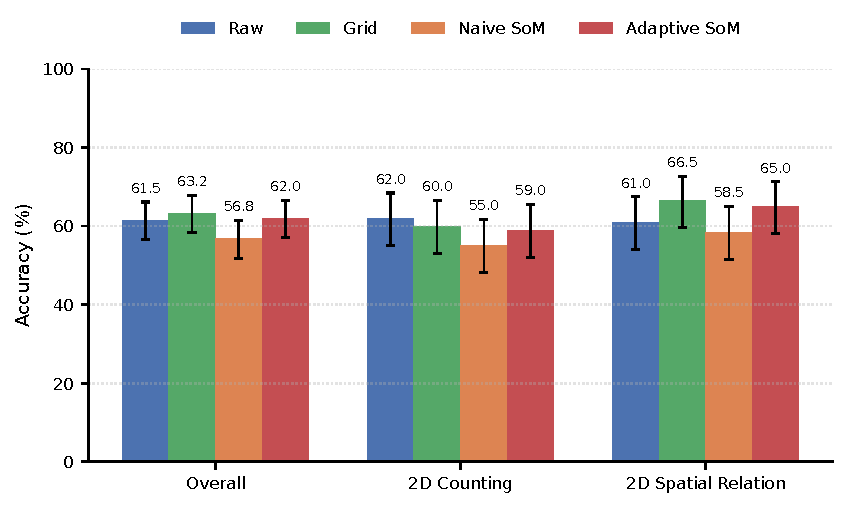
\includegraphics[width=0.98\textwidth]{figures/fig2_main_accuracy.pdf}
\caption{Accuracy by task with 95\% Wilson intervals. The Grid is strongest on spatial relation; no detector-based SoM beats Raw on counting.}
\label{fig:main}
\end{figure*}

\begin{table}[t]
\centering
\footnotesize
\setlength{\tabcolsep}{2.4pt}
\begin{tabular}{lcccccc}
\toprule
Density & $n$ & Raw & Grid & Naive & Adaptive & $p$ \\
\midrule
Low & 135 & 58.5 & \best{63.0} & 57.8 & 60.0 & 0.5488 \\
Medium & 145 & \best{60.0} & 58.6 & 49.7 & \best{60.0} & 0.0015 \\
High & 120 & 66.7 & \best{69.2} & 64.2 & 66.7 & 0.6291 \\
\bottomrule
\end{tabular}
\caption{Accuracy (\%) by detected-object density. $p$ is the exact McNemar test for Adaptive vs naive SoM within the bucket. Grid is included so the table matches Figure~\ref{fig:density}; the best value per row is bold.}
\label{tab:density}
\end{table}

\paragraph{Task--prompt decoupling.}
Table~\ref{tab:main} shows that the Grid is the strongest condition on 2D spatial relation (66.5\% vs.\ Raw 61.0\%), and the strongest overall (63.2\%). In contrast, all detector-based marks remain below Raw on 2D counting: Raw 62.0\%, Adaptive 59.0\%, Naive 55.0\%, Grid 60.0\%. The pattern is consistent with \emph{task--prompt decoupling}: coordinate structure helps relational reasoning, whereas marks tuned to object proposals do not help counting on this model and can hurt it.

\paragraph{Occlusion trade-off and class-agnostic distraction.}
Naive SoM significantly degrades overall accuracy relative to Raw (56.8\% vs.\ 61.5\%, $p=0.0163$). Adaptive SoM recovers most of that loss (62.0\% vs.\ 56.8\%, $p=0.0038$), but does not exceed Raw ($p=0.8642$). Table~\ref{tab:density} localizes the effect: at medium density, Adaptive SoM reaches 60.0\% versus 49.7\% for Naive SoM ($p=0.0015$); at high density the two are closer (66.7\% vs.\ 64.2\%, $p=0.6291$), and Grid is strongest (69.2\%). Density reduction is necessary but not sufficient when the detector itself is unreliable. Because YOLOv8n is class-agnostic in our pipeline, it can label irrelevant objects (Figure~\ref{fig:cases}, bottom-left), which distracts the model even when the overlay is thin.

\begin{figure}[t]
\centering
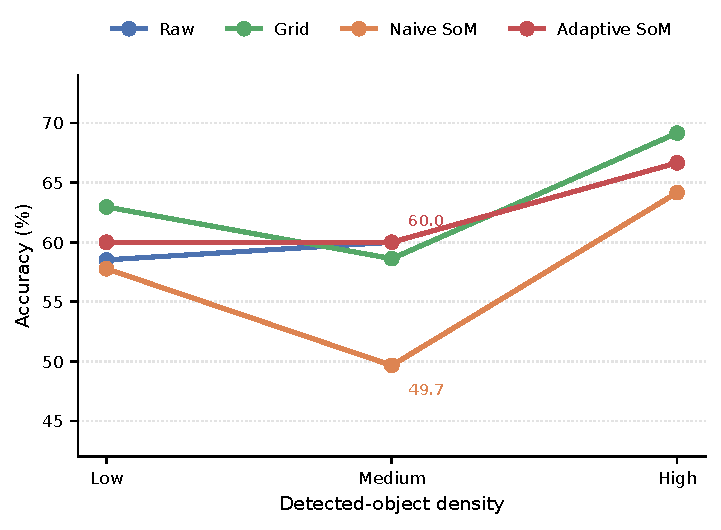
\includegraphics[width=0.98\columnwidth]{figures/fig3_density_tradeoff.pdf}
\caption{Accuracy across low, medium, and high detected-object density. The y-axis is truncated to 42--74\% to make the 49.7\% medium-density drop of Naive SoM and the 60.0\% recovery of Adaptive SoM visible; the full range is 0--100\%.}
\label{fig:density}
\end{figure}

\begin{figure*}[t]
\centering
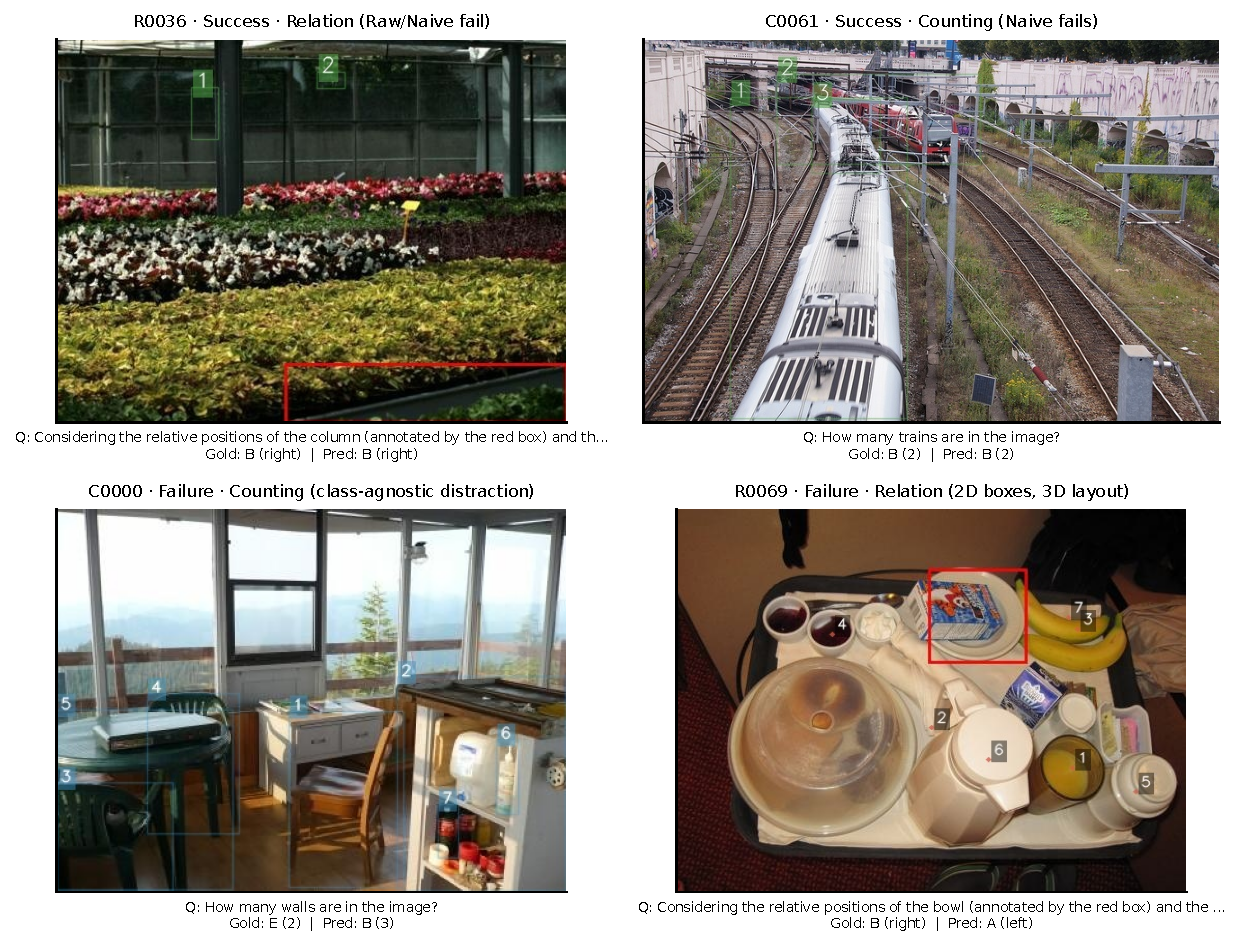
\includegraphics[width=0.98\textwidth]{figures/fig4_qualitative_cases.pdf}
\caption{Curated qualitative cases: two 2D Relation and two 2D Counting examples. Top-left (R0036): Raw and Naive SoM fail while Grid and Adaptive SoM answer the relation correctly. Top-right (C0061): Naive SoM over-labels and fails on counting, while Adaptive SoM succeeds. Bottom-left (C0000): a class-agnostic detector places marks on walls/furniture, illustrating detector distraction. Bottom-right (R0069): a 2D box cannot express the tabletop layout needed for the relation. Each panel shows the question and both the option letter and its text.}
\label{fig:cases}
\end{figure*}

\paragraph{Failure analysis.}
Two failure modes dominate. First, the detector can miss a small object, so no mark is placed and the model has to count from the raw image. Second, a contour fallback may merge adjacent objects into one proposal, producing a misleading count. Spatial relation questions also fail when the relation depends on 3D layout or occlusion cues that a 2D box cannot express. These failures are reported rather than filtered: the method improves the annotation policy, not the detector or the model's visual prior.

\paragraph{Cost.}
The detector and renderer are offline and run once per image. Inference cost is dominated by the 2B MLLM; mean latency is 0.31\,s for Raw and 0.32\,s for Adaptive SoM, with peak allocated memory 4437\,MB (4.4\,GB). No training, fine-tuning, or additional parameters are introduced.

\section{Conclusion and Limitations}
\label{sec:conclusion}
We presented a diagnostic study of training-free visual prompting for edge MLLMs, not a new state-of-the-art claim. On a fixed 400-question CV-Bench 2D subset, we find task--prompt decoupling: a simple coordinate Grid improves spatial relation (66.5\% vs.\ 61.0\%) and is strongest overall (63.2\%), while no detector-based SoM beats Raw on counting (62.0\%). We also find an occlusion trade-off and a detector-distraction bottleneck: fixed Naive SoM significantly hurts (56.8\% vs.\ 61.5\%), density-aware rendering recovers most of the loss (62.0\%, $p=0.0038$ vs.\ Naive; medium 60.0\% vs.\ 49.7\%), but cannot surpass Raw or repair labels placed on irrelevant objects. The study is limited to one 2B base model, one benchmark subset, and 2D tasks; extending it to multiple base models, 3D relations, and detector-aware proposal filtering is future work.

\bibliographystyle{plain}
\bibliography{references}

\end{document}
